\documentclass[twoside]{book}

% Packages required by doxygen
\usepackage{fixltx2e}
\usepackage{calc}
\usepackage{doxygen}
\usepackage[export]{adjustbox} % also loads graphicx
\usepackage{graphicx}
\usepackage[utf8]{inputenc}
\usepackage{makeidx}
\usepackage{multicol}
\usepackage{multirow}
\PassOptionsToPackage{warn}{textcomp}
\usepackage{textcomp}
\usepackage[nointegrals]{wasysym}
\usepackage[table]{xcolor}

% Font selection
\usepackage[T1]{fontenc}
\usepackage[scaled=.90]{helvet}
\usepackage{courier}
\usepackage{amssymb}
\usepackage{sectsty}
\renewcommand{\familydefault}{\sfdefault}
\allsectionsfont{%
  \fontseries{bc}\selectfont%
  \color{darkgray}%
}
\renewcommand{\DoxyLabelFont}{%
  \fontseries{bc}\selectfont%
  \color{darkgray}%
}
\newcommand{\+}{\discretionary{\mbox{\scriptsize$\hookleftarrow$}}{}{}}

% Page & text layout
\usepackage{geometry}
\geometry{%
  a4paper,%
  top=2.5cm,%
  bottom=2.5cm,%
  left=2.5cm,%
  right=2.5cm%
}
\tolerance=750
\hfuzz=15pt
\hbadness=750
\setlength{\emergencystretch}{15pt}
\setlength{\parindent}{0cm}
\setlength{\parskip}{0.2cm}
\makeatletter
\renewcommand{\paragraph}{%
  \@startsection{paragraph}{4}{0ex}{-1.0ex}{1.0ex}{%
    \normalfont\normalsize\bfseries\SS@parafont%
  }%
}
\renewcommand{\subparagraph}{%
  \@startsection{subparagraph}{5}{0ex}{-1.0ex}{1.0ex}{%
    \normalfont\normalsize\bfseries\SS@subparafont%
  }%
}
\makeatother

% Headers & footers
\usepackage{fancyhdr}
\pagestyle{fancyplain}
\fancyhead[LE]{\fancyplain{}{\bfseries\thepage}}
\fancyhead[CE]{\fancyplain{}{}}
\fancyhead[RE]{\fancyplain{}{\bfseries\leftmark}}
\fancyhead[LO]{\fancyplain{}{\bfseries\rightmark}}
\fancyhead[CO]{\fancyplain{}{}}
\fancyhead[RO]{\fancyplain{}{\bfseries\thepage}}
\fancyfoot[LE]{\fancyplain{}{}}
\fancyfoot[CE]{\fancyplain{}{}}
\fancyfoot[RE]{\fancyplain{}{\bfseries\scriptsize Generated on Wed Aug 19 2015 12\+:26\+:52 for archived by Doxygen }}
\fancyfoot[LO]{\fancyplain{}{\bfseries\scriptsize Generated on Wed Aug 19 2015 12\+:26\+:52 for archived by Doxygen }}
\fancyfoot[CO]{\fancyplain{}{}}
\fancyfoot[RO]{\fancyplain{}{}}
\renewcommand{\footrulewidth}{0.4pt}
\renewcommand{\chaptermark}[1]{%
  \markboth{#1}{}%
}
\renewcommand{\sectionmark}[1]{%
  \markright{\thesection\ #1}%
}

% Indices & bibliography
\usepackage{natbib}
\usepackage[titles]{tocloft}
\setcounter{tocdepth}{3}
\setcounter{secnumdepth}{5}
\makeindex

% Hyperlinks (required, but should be loaded last)
\usepackage{ifpdf}
\ifpdf
  \usepackage[pdftex,pagebackref=true]{hyperref}
\else
  \usepackage[ps2pdf,pagebackref=true]{hyperref}
\fi
\hypersetup{%
  colorlinks=true,%
  linkcolor=blue,%
  citecolor=blue,%
  unicode%
}

% Custom commands
\newcommand{\clearemptydoublepage}{%
  \newpage{\pagestyle{empty}\cleardoublepage}%
}


%===== C O N T E N T S =====

\begin{document}

% Titlepage & ToC
\hypersetup{pageanchor=false,
             bookmarks=true,
             bookmarksnumbered=true,
             pdfencoding=unicode
            }
\pagenumbering{roman}
\begin{titlepage}
\vspace*{7cm}
\begin{center}%
{\Large archived }\\
\vspace*{1cm}
{\large Generated by Doxygen 1.8.9.1}\\
\vspace*{0.5cm}
{\small Wed Aug 19 2015 12:26:52}\\
\end{center}
\end{titlepage}
\clearemptydoublepage
\tableofcontents
\clearemptydoublepage
\pagenumbering{arabic}
\hypersetup{pageanchor=true}

%--- Begin generated contents ---
\chapter{Hierarchical Index}
\section{Class Hierarchy}
This inheritance list is sorted roughly, but not completely, alphabetically\+:\begin{DoxyCompactList}
\item \contentsline{section}{archived$<$ Value $>$}{\pageref{classarchived}}{}
\item pair\begin{DoxyCompactList}
\item \contentsline{section}{archived$<$ Value $>$\+:\+:commit}{\pageref{classarchived_1_1commit}}{}
\end{DoxyCompactList}
\item \contentsline{section}{archived$<$ Value $>$\+:\+:version}{\pageref{classarchived_1_1version}}{}
\end{DoxyCompactList}

\chapter{Class Index}
\section{Class List}
Here are the classes, structs, unions and interfaces with brief descriptions\+:\begin{DoxyCompactList}
\item\contentsline{section}{\hyperlink{classarchived}{archived$<$ Value $>$} \\*A class to keep track of an incrementally updated variable }{\pageref{classarchived}}{}
\item\contentsline{section}{\hyperlink{classarchived_1_1version}{archived$<$ Value $>$\+::version} \\*A version of an archived$<$$>$ }{\pageref{classarchived_1_1version}}{}
\end{DoxyCompactList}

\chapter{File Index}
\section{File List}
Here is a list of all files with brief descriptions\+:\begin{DoxyCompactList}
\item\contentsline{section}{\hyperlink{archived_8h}{archived.\+h} }{\pageref{archived_8h}}{}
\item\contentsline{section}{\hyperlink{archived__test_8cpp}{archived\+\_\+test.\+cpp} }{\pageref{archived__test_8cpp}}{}
\end{DoxyCompactList}

\chapter{Class Documentation}
\hypertarget{classarchived}{}\section{archived$<$ Value $>$ Class Template Reference}
\label{classarchived}\index{archived$<$ Value $>$@{archived$<$ Value $>$}}


A class to keep track of an incrementally updated variable.  




{\ttfamily \#include $<$archived.\+h$>$}

\subsection*{Classes}
\begin{DoxyCompactItemize}
\item 
class \hyperlink{classarchived_1_1version}{version}
\begin{DoxyCompactList}\small\item\em A version of an archived$<$$>$ \end{DoxyCompactList}\end{DoxyCompactItemize}
\subsection*{Public Types}
\begin{DoxyCompactItemize}
\item 
\hypertarget{classarchived_a0f6c13c55e504fe3bbfc04f3896e5abc}{}typedef Value \hyperlink{classarchived_a0f6c13c55e504fe3bbfc04f3896e5abc}{value\+\_\+type}\label{classarchived_a0f6c13c55e504fe3bbfc04f3896e5abc}

\begin{DoxyCompactList}\small\item\em The archived value\textquotesingle{}s type. \end{DoxyCompactList}\item 
\hypertarget{classarchived_a75b8e571e7c6aca9432b9aa2ba601c00}{}typedef \hyperlink{classarchived_1_1version}{version} \hyperlink{classarchived_a75b8e571e7c6aca9432b9aa2ba601c00}{version\+\_\+type}\label{classarchived_a75b8e571e7c6aca9432b9aa2ba601c00}

\begin{DoxyCompactList}\small\item\em The type of versions provided. \end{DoxyCompactList}\end{DoxyCompactItemize}
\subsection*{Public Member Functions}
\begin{DoxyCompactItemize}
\item 
\hyperlink{classarchived_a752f1c457d9431caab148b866fc34c0f}{archived} (const \hyperlink{classarchived_a0f6c13c55e504fe3bbfc04f3896e5abc}{value\+\_\+type} \&initial\+\_\+value)
\begin{DoxyCompactList}\small\item\em Constructor that initializes the archived$<$$>$ with initial\+\_\+value. After construction, the archived$<$$>$\textquotesingle{}s current value is initial\+\_\+value. \end{DoxyCompactList}\item 
\hyperlink{classarchived_a75b8e571e7c6aca9432b9aa2ba601c00}{version\+\_\+type} \hyperlink{classarchived_a8d1c7030894bf31b7add0bccd041d69a}{increment\+\_\+by} (const \hyperlink{classarchived_a0f6c13c55e504fe3bbfc04f3896e5abc}{value\+\_\+type} \&increment)
\begin{DoxyCompactList}\small\item\em Increments the value by increment. Uses operator+= on the value. Returns a new version. \end{DoxyCompactList}\item 
\hyperlink{classarchived_a0f6c13c55e504fe3bbfc04f3896e5abc}{value\+\_\+type} \hyperlink{classarchived_af69a2753a3b9844609a4b2684e4e0bf3}{value} () const 
\begin{DoxyCompactList}\small\item\em Returns the current value. \end{DoxyCompactList}\item 
\hyperlink{classarchived_a75b8e571e7c6aca9432b9aa2ba601c00}{version\+\_\+type} \hyperlink{classarchived_a5af939f79bddf33f8773fcb89016a85d}{clear\+\_\+history} ()
\begin{DoxyCompactList}\small\item\em Clears the stored history data. Leaves current value unchanged. All associated versions are invalidated. Returns a new (valid) version. \end{DoxyCompactList}\item 
\hyperlink{classarchived_a75b8e571e7c6aca9432b9aa2ba601c00}{version\+\_\+type} \hyperlink{classarchived_ae76263bf1bcd3dd0f6023c8142691a6c}{reset} (const \hyperlink{classarchived_a0f6c13c55e504fe3bbfc04f3896e5abc}{value\+\_\+type} \&initial\+\_\+value)
\begin{DoxyCompactList}\small\item\em Clears the stored history data. Sets current value to initial\+\_\+value. All associated versions are invalidated. Returns a new (valid) version. \end{DoxyCompactList}\item 
\hyperlink{classarchived_a75b8e571e7c6aca9432b9aa2ba601c00}{version\+\_\+type} \hyperlink{classarchived_a7b7505259596c1deaff30a9fb7942bb5}{current} () const 
\begin{DoxyCompactList}\small\item\em Returns a new version. \end{DoxyCompactList}\end{DoxyCompactItemize}


\subsection{Detailed Description}
\subsubsection*{template$<$class Value$>$class archived$<$ Value $>$}

A class to keep track of an incrementally updated variable. 

\subsection*{Overview}

The class archived$<$\+Value$>$ keeps track of a variable of type Value that is incrementally upgraded.

It is possible to retrieve intermediate versions, which later on allow a computation of the difference between that version and the current version.

\subsubsection*{Versions\+:}

An archived$<$$>$ provides the concept of a version. A version is associated with the archived$<$$>$ that created it. A version has a validity, it is either valid or invalid.

A version is only valid as long as the associated archived$<$$>$ exists.

Valid versions can be used to compute the difference between the value of the associated archived$<$$>$ at creation time of the version and the current one.

A version is valid when acquired via an archived$<$$>$, but can be invalidated by certain actions on the associated archived$<$$>$. 

\subsection{Constructor \& Destructor Documentation}
\hypertarget{classarchived_a752f1c457d9431caab148b866fc34c0f}{}\index{archived@{archived}!archived@{archived}}
\index{archived@{archived}!archived@{archived}}
\subsubsection[{archived}]{\setlength{\rightskip}{0pt plus 5cm}template$<$class Value $>$ {\bf archived}$<$ Value $>$\+::{\bf archived} (
\begin{DoxyParamCaption}
\item[{const {\bf value\+\_\+type} \&}]{initial\+\_\+value}
\end{DoxyParamCaption}
)\hspace{0.3cm}{\ttfamily [explicit]}}\label{classarchived_a752f1c457d9431caab148b866fc34c0f}


Constructor that initializes the archived$<$$>$ with initial\+\_\+value. After construction, the archived$<$$>$\textquotesingle{}s current value is initial\+\_\+value. 


\begin{DoxyParams}{Parameters}
{\em initial\+\_\+value} & The initial value. \\
\hline
\end{DoxyParams}


\subsection{Member Function Documentation}
\hypertarget{classarchived_a5af939f79bddf33f8773fcb89016a85d}{}\index{archived@{archived}!clear\+\_\+history@{clear\+\_\+history}}
\index{clear\+\_\+history@{clear\+\_\+history}!archived@{archived}}
\subsubsection[{clear\+\_\+history}]{\setlength{\rightskip}{0pt plus 5cm}template$<$class Value $>$ {\bf archived}$<$ Value $>$\+::{\bf version\+\_\+type} {\bf archived}$<$ Value $>$\+::clear\+\_\+history (
\begin{DoxyParamCaption}
{}
\end{DoxyParamCaption}
)}\label{classarchived_a5af939f79bddf33f8773fcb89016a85d}


Clears the stored history data. Leaves current value unchanged. All associated versions are invalidated. Returns a new (valid) version. 

\begin{DoxyReturn}{Returns}
A new version. 
\end{DoxyReturn}
\hypertarget{classarchived_a7b7505259596c1deaff30a9fb7942bb5}{}\index{archived@{archived}!current@{current}}
\index{current@{current}!archived@{archived}}
\subsubsection[{current}]{\setlength{\rightskip}{0pt plus 5cm}template$<$class Value $>$ {\bf archived}$<$ Value $>$\+::{\bf version\+\_\+type} {\bf archived}$<$ Value $>$\+::current (
\begin{DoxyParamCaption}
{}
\end{DoxyParamCaption}
) const}\label{classarchived_a7b7505259596c1deaff30a9fb7942bb5}


Returns a new version. 

\begin{DoxyReturn}{Returns}
A new version. 
\end{DoxyReturn}
\hypertarget{classarchived_a8d1c7030894bf31b7add0bccd041d69a}{}\index{archived@{archived}!increment\+\_\+by@{increment\+\_\+by}}
\index{increment\+\_\+by@{increment\+\_\+by}!archived@{archived}}
\subsubsection[{increment\+\_\+by}]{\setlength{\rightskip}{0pt plus 5cm}template$<$class Value$>$ {\bf archived}$<$ Value $>$\+::{\bf version\+\_\+type} {\bf archived}$<$ Value $>$\+::increment\+\_\+by (
\begin{DoxyParamCaption}
\item[{const {\bf value\+\_\+type} \&}]{increment}
\end{DoxyParamCaption}
)}\label{classarchived_a8d1c7030894bf31b7add0bccd041d69a}


Increments the value by increment. Uses operator+= on the value. Returns a new version. 

\begin{DoxyReturn}{Returns}
A new version. 
\end{DoxyReturn}

\begin{DoxyParams}{Parameters}
{\em increment} & The value to increment by. \\
\hline
\end{DoxyParams}
\hypertarget{classarchived_ae76263bf1bcd3dd0f6023c8142691a6c}{}\index{archived@{archived}!reset@{reset}}
\index{reset@{reset}!archived@{archived}}
\subsubsection[{reset}]{\setlength{\rightskip}{0pt plus 5cm}template$<$class Value$>$ {\bf archived}$<$ Value $>$\+::{\bf version\+\_\+type} {\bf archived}$<$ Value $>$\+::reset (
\begin{DoxyParamCaption}
\item[{const {\bf value\+\_\+type} \&}]{initial\+\_\+value}
\end{DoxyParamCaption}
)}\label{classarchived_ae76263bf1bcd3dd0f6023c8142691a6c}


Clears the stored history data. Sets current value to initial\+\_\+value. All associated versions are invalidated. Returns a new (valid) version. 

\begin{DoxyReturn}{Returns}
A new version. 
\end{DoxyReturn}

\begin{DoxyParams}{Parameters}
{\em initial\+\_\+value} & The new value. \\
\hline
\end{DoxyParams}
\hypertarget{classarchived_af69a2753a3b9844609a4b2684e4e0bf3}{}\index{archived@{archived}!value@{value}}
\index{value@{value}!archived@{archived}}
\subsubsection[{value}]{\setlength{\rightskip}{0pt plus 5cm}template$<$class Value $>$ {\bf archived}$<$ Value $>$\+::{\bf value\+\_\+type} {\bf archived}$<$ Value $>$\+::value (
\begin{DoxyParamCaption}
{}
\end{DoxyParamCaption}
) const}\label{classarchived_af69a2753a3b9844609a4b2684e4e0bf3}


Returns the current value. 

\begin{DoxyReturn}{Returns}
the current value. 
\end{DoxyReturn}


The documentation for this class was generated from the following file\+:\begin{DoxyCompactItemize}
\item 
\hyperlink{archived_8h}{archived.\+h}\end{DoxyCompactItemize}

\hypertarget{classarchived_1_1commit}{}\section{archived$<$ Value $>$\+:\+:commit Class Reference}
\label{classarchived_1_1commit}\index{archived$<$ Value $>$\+::commit@{archived$<$ Value $>$\+::commit}}


A commit is an atomic diff. It contains an iterator to its successor and the value of the diff.  




{\ttfamily \#include $<$archived.\+h$>$}

Inheritance diagram for archived$<$ Value $>$\+:\+:commit\+:\begin{figure}[H]
\begin{center}
\leavevmode
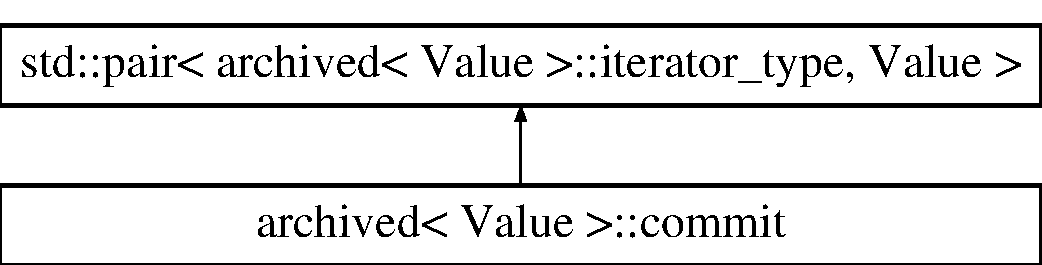
\includegraphics[height=2.000000cm]{classarchived_1_1commit}
\end{center}
\end{figure}


\subsection{Detailed Description}
\subsubsection*{template$<$class Value$>$class archived$<$ Value $>$\+::commit}

A commit is an atomic diff. It contains an iterator to its successor and the value of the diff. 



The documentation for this class was generated from the following file\+:\begin{DoxyCompactItemize}
\item 
\hyperlink{archived_8h}{archived.\+h}\end{DoxyCompactItemize}

\hypertarget{classarchived_1_1version}{}\section{archived$<$ Value $>$\+:\+:version Class Reference}
\label{classarchived_1_1version}\index{archived$<$ Value $>$\+::version@{archived$<$ Value $>$\+::version}}


A version of an archived$<$$>$  




{\ttfamily \#include $<$archived.\+h$>$}

\subsection*{Public Types}
\begin{DoxyCompactItemize}
\item 
\hypertarget{classarchived_1_1version_ae9028b053631ebb7832c9457cac4c29b}{}typedef Value \hyperlink{classarchived_1_1version_ae9028b053631ebb7832c9457cac4c29b}{value\+\_\+type}\label{classarchived_1_1version_ae9028b053631ebb7832c9457cac4c29b}

\begin{DoxyCompactList}\small\item\em The associated archived value\textquotesingle{}s type. \end{DoxyCompactList}\item 
\hypertarget{classarchived_1_1version_a791c80c76addc75c5ee41f31ae41817a}{}typedef \hyperlink{classarchived}{archived}$<$ Value $>$ \hyperlink{classarchived_1_1version_a791c80c76addc75c5ee41f31ae41817a}{archive\+\_\+type}\label{classarchived_1_1version_a791c80c76addc75c5ee41f31ae41817a}

\begin{DoxyCompactList}\small\item\em The associated archived\textquotesingle{}s type. \end{DoxyCompactList}\end{DoxyCompactItemize}
\subsection*{Public Member Functions}
\begin{DoxyCompactItemize}
\item 
\hypertarget{classarchived_1_1version_a75950e89fdd7d100d9bb9c52be9750e5}{}\hyperlink{classarchived_1_1version_a75950e89fdd7d100d9bb9c52be9750e5}{version} ()\label{classarchived_1_1version_a75950e89fdd7d100d9bb9c52be9750e5}

\begin{DoxyCompactList}\small\item\em Default Constructor. A default constructed version is not valid. \end{DoxyCompactList}\item 
\hyperlink{classarchived_1_1version_ac511988e424b10abf26638b9aeb49934}{version} (const \hyperlink{classarchived_1_1version}{version} \&other)=default
\begin{DoxyCompactList}\small\item\em Default Copy Constructor A copy constructed version has the same same properties as the source. \end{DoxyCompactList}\item 
\hyperlink{classarchived_1_1version_a554be7a467115e99c8f2b6ea4aa8ea2d}{version} (\hyperlink{classarchived_1_1version}{version} \&\&other)=default
\begin{DoxyCompactList}\small\item\em Default Move Constructor A move constructed version has the same same properties as the source. \end{DoxyCompactList}\item 
\hyperlink{classarchived_1_1version}{version} \& \hyperlink{classarchived_1_1version_aa808a277ce1c999ac7472aaa1d77a7e3}{operator=} (const \hyperlink{classarchived_1_1version}{version} \&other)=default
\begin{DoxyCompactList}\small\item\em Default Assignment operator Copies from other. An assigned version has the same same properties as the source. \end{DoxyCompactList}\item 
\hyperlink{classarchived_1_1version}{version} \& \hyperlink{classarchived_1_1version_a8f5347b0b1207478ac2ec6219e5c315d}{operator=} (\hyperlink{classarchived_1_1version}{version} \&\&other)=default
\begin{DoxyCompactList}\small\item\em Default Move Assignment operator Moves from other. A move assigned version has the same same properties as the source. \end{DoxyCompactList}\end{DoxyCompactItemize}


\subsection{Detailed Description}
\subsubsection*{template$<$class Value$>$class archived$<$ Value $>$\+::version}

A version of an archived$<$$>$ 

An archived$<$$>$ provides the concept of a version. A version is associated with the archived$<$$>$ that created it. A version has a validity, it is either valid or invalid.

A version is only valid as long as the associated archived$<$$>$ exists.

Valid versions can be used to compute the difference between the value of the associated archived$<$$>$ at creation time of the version and the current one.

A version is valid when acquired via an archived$<$$>$, but can be invalidated by certain actions on the associated archived$<$$>$. 

\subsection{Constructor \& Destructor Documentation}
\hypertarget{classarchived_1_1version_ac511988e424b10abf26638b9aeb49934}{}\index{archived\+::version@{archived\+::version}!version@{version}}
\index{version@{version}!archived\+::version@{archived\+::version}}
\subsubsection[{version}]{\setlength{\rightskip}{0pt plus 5cm}template$<$class Value$>$ {\bf archived}$<$ Value $>$\+::version\+::version (
\begin{DoxyParamCaption}
\item[{const {\bf version} \&}]{other}
\end{DoxyParamCaption}
)\hspace{0.3cm}{\ttfamily [default]}}\label{classarchived_1_1version_ac511988e424b10abf26638b9aeb49934}


Default Copy Constructor A copy constructed version has the same same properties as the source. 


\begin{DoxyParams}{Parameters}
{\em other} & The source of the copy. \\
\hline
\end{DoxyParams}
\hypertarget{classarchived_1_1version_a554be7a467115e99c8f2b6ea4aa8ea2d}{}\index{archived\+::version@{archived\+::version}!version@{version}}
\index{version@{version}!archived\+::version@{archived\+::version}}
\subsubsection[{version}]{\setlength{\rightskip}{0pt plus 5cm}template$<$class Value$>$ {\bf archived}$<$ Value $>$\+::version\+::version (
\begin{DoxyParamCaption}
\item[{{\bf version} \&\&}]{other}
\end{DoxyParamCaption}
)\hspace{0.3cm}{\ttfamily [default]}}\label{classarchived_1_1version_a554be7a467115e99c8f2b6ea4aa8ea2d}


Default Move Constructor A move constructed version has the same same properties as the source. 


\begin{DoxyParams}{Parameters}
{\em other} & The source of the move. \\
\hline
\end{DoxyParams}


\subsection{Member Function Documentation}
\hypertarget{classarchived_1_1version_aa808a277ce1c999ac7472aaa1d77a7e3}{}\index{archived\+::version@{archived\+::version}!operator=@{operator=}}
\index{operator=@{operator=}!archived\+::version@{archived\+::version}}
\subsubsection[{operator=}]{\setlength{\rightskip}{0pt plus 5cm}template$<$class Value$>$ {\bf version}\& {\bf archived}$<$ Value $>$\+::version\+::operator= (
\begin{DoxyParamCaption}
\item[{const {\bf version} \&}]{other}
\end{DoxyParamCaption}
)\hspace{0.3cm}{\ttfamily [default]}}\label{classarchived_1_1version_aa808a277ce1c999ac7472aaa1d77a7e3}


Default Assignment operator Copies from other. An assigned version has the same same properties as the source. 

\begin{DoxyReturn}{Returns}
A reference to $\ast$this 
\end{DoxyReturn}

\begin{DoxyParams}{Parameters}
{\em other} & The source of the copy. \\
\hline
\end{DoxyParams}
\hypertarget{classarchived_1_1version_a8f5347b0b1207478ac2ec6219e5c315d}{}\index{archived\+::version@{archived\+::version}!operator=@{operator=}}
\index{operator=@{operator=}!archived\+::version@{archived\+::version}}
\subsubsection[{operator=}]{\setlength{\rightskip}{0pt plus 5cm}template$<$class Value$>$ {\bf version}\& {\bf archived}$<$ Value $>$\+::version\+::operator= (
\begin{DoxyParamCaption}
\item[{{\bf version} \&\&}]{other}
\end{DoxyParamCaption}
)\hspace{0.3cm}{\ttfamily [default]}}\label{classarchived_1_1version_a8f5347b0b1207478ac2ec6219e5c315d}


Default Move Assignment operator Moves from other. A move assigned version has the same same properties as the source. 

\begin{DoxyReturn}{Returns}
A reference to $\ast$this 
\end{DoxyReturn}

\begin{DoxyParams}{Parameters}
{\em other} & The source of the copy. \\
\hline
\end{DoxyParams}


The documentation for this class was generated from the following file\+:\begin{DoxyCompactItemize}
\item 
\hyperlink{archived_8h}{archived.\+h}\end{DoxyCompactItemize}

\chapter{File Documentation}
\hypertarget{archived_8h}{}\section{archived.\+h File Reference}
\label{archived_8h}\index{archived.\+h@{archived.\+h}}
{\ttfamily \#include $<$forward\+\_\+list$>$}\\*
\subsection*{Classes}
\begin{DoxyCompactItemize}
\item 
class \hyperlink{classarchived}{archived$<$ Value $>$}
\begin{DoxyCompactList}\small\item\em A class to keep track of an incrementally updated variable. \end{DoxyCompactList}\item 
class \hyperlink{classarchived_1_1version}{archived$<$ Value $>$\+::version}
\begin{DoxyCompactList}\small\item\em A version of an archived$<$$>$ \end{DoxyCompactList}\end{DoxyCompactItemize}
\subsection*{Functions}
\begin{DoxyCompactItemize}
\item 
{\footnotesize template$<$class Version $>$ }\\Version\+::value\+\_\+type \hyperlink{archived_8h_a0069eef7ac554f43a4fff498c02c2d01}{diff\+\_\+to\+\_\+current} (const Version \&old)
\begin{DoxyCompactList}\small\item\em Computes the difference of old and current value. \end{DoxyCompactList}\end{DoxyCompactItemize}


\subsection{Function Documentation}
\hypertarget{archived_8h_a0069eef7ac554f43a4fff498c02c2d01}{}\index{archived.\+h@{archived.\+h}!diff\+\_\+to\+\_\+current@{diff\+\_\+to\+\_\+current}}
\index{diff\+\_\+to\+\_\+current@{diff\+\_\+to\+\_\+current}!archived.\+h@{archived.\+h}}
\subsubsection[{diff\+\_\+to\+\_\+current}]{\setlength{\rightskip}{0pt plus 5cm}template$<$class Version $>$ Version\+::value\+\_\+type diff\+\_\+to\+\_\+current (
\begin{DoxyParamCaption}
\item[{const Version \&}]{old}
\end{DoxyParamCaption}
)}\label{archived_8h_a0069eef7ac554f43a4fff498c02c2d01}


Computes the difference of old and current value. 

This function computes the accumulated increments of the archived$<$$>$ associated with old from old\textquotesingle{}s creation time to present.

\begin{DoxyReturn}{Returns}
The value difference between old and current version. 
\end{DoxyReturn}

\begin{DoxyParams}{Parameters}
{\em old} & An old Version. \\
\hline
\end{DoxyParams}

\hypertarget{archived__test_8cpp}{}\section{archived\+\_\+test.\+cpp File Reference}
\label{archived__test_8cpp}\index{archived\+\_\+test.\+cpp@{archived\+\_\+test.\+cpp}}
{\ttfamily \#include \char`\"{}archived.\+h\char`\"{}}\\*
{\ttfamily \#include $<$vector$>$}\\*
{\ttfamily \#include $<$numeric$>$}\\*
{\ttfamily \#include $<$iostream$>$}\\*
\subsection*{Functions}
\begin{DoxyCompactItemize}
\item 
bool \hyperlink{archived__test_8cpp_a33029416565d9a65a4daf83aecdbd0bb}{check\+\_\+equal} (int a, int b, const std\+::string \&msg)
\item 
int \hyperlink{archived__test_8cpp_a217dbf8b442f20279ea00b898af96f52}{main} (int argc, const char $\ast$$\ast$argv)
\end{DoxyCompactItemize}


\subsection{Function Documentation}
\hypertarget{archived__test_8cpp_a33029416565d9a65a4daf83aecdbd0bb}{}\index{archived\+\_\+test.\+cpp@{archived\+\_\+test.\+cpp}!check\+\_\+equal@{check\+\_\+equal}}
\index{check\+\_\+equal@{check\+\_\+equal}!archived\+\_\+test.\+cpp@{archived\+\_\+test.\+cpp}}
\subsubsection[{check\+\_\+equal}]{\setlength{\rightskip}{0pt plus 5cm}bool check\+\_\+equal (
\begin{DoxyParamCaption}
\item[{int}]{a, }
\item[{int}]{b, }
\item[{const std\+::string \&}]{msg}
\end{DoxyParamCaption}
)}\label{archived__test_8cpp_a33029416565d9a65a4daf83aecdbd0bb}
\hypertarget{archived__test_8cpp_a217dbf8b442f20279ea00b898af96f52}{}\index{archived\+\_\+test.\+cpp@{archived\+\_\+test.\+cpp}!main@{main}}
\index{main@{main}!archived\+\_\+test.\+cpp@{archived\+\_\+test.\+cpp}}
\subsubsection[{main}]{\setlength{\rightskip}{0pt plus 5cm}int main (
\begin{DoxyParamCaption}
\item[{int}]{argc, }
\item[{const char $\ast$$\ast$}]{argv}
\end{DoxyParamCaption}
)}\label{archived__test_8cpp_a217dbf8b442f20279ea00b898af96f52}

%--- End generated contents ---

% Index
\backmatter
\newpage
\phantomsection
\clearemptydoublepage
\addcontentsline{toc}{chapter}{Index}
\printindex

\end{document}
